\documentclass[12pt,a4paper]{report}

\usepackage[a4paper,margin=1in]{geometry}
\usepackage{graphicx}
\usepackage{hyperref}
\usepackage{float}
\usepackage{setspace}

\setlength{\parindent}{0pt}
\setlength{\parskip}{6pt}
\onehalfspacing

\title{COMP4135 SEM Weekly Report 1}
\author{Group 2}
\date{19/03/2026}

\begin{document}

\begin{titlepage}
\centering

\includegraphics[width=0.45\textwidth]{media/image1.png}\par
\vspace{1.5cm}
{\LARGE \textbf{COMP4135 SEM Weekly Report 1}\par}
\vspace{0.6cm}
{\Large \textbf{Group 2}\par}
\vspace{1cm}
{\large \textbf{Team members:}\par}
\vspace{0.5cm}
{\large Guangjun HU (20511787)\par}
{\large Hongshuo HU (20808603)\par}
{\large Cheng YE (20513323)\par}
{\large Zehan CHEN (20807750)\par}
\vfill
{\large School of Computer Science University of Nottingham\par}
\vspace{0.5cm}
{\large Submission Date: 19/03/2026\par}
\end{titlepage}

\tableofcontents
\clearpage

\chapter{Introduction}

This weekly report is the very first one for this Unity game project. It mainly clarifies the division of people resource among project members and the project direction.

\section{Description}

This project is a group coursework of the Software Engineering Management module, which aims to design, develop, and test a game based on Unity. The core assignment focuses on documenting and collaborating. Our initial game direction candidate includes board chess game, complex card game (War of the Three Kingdoms). And we finally determined the direction of our game, Tactical Cards. It combines the grid based movement of board chess game with using cards to control from the card game, resulting a turn based strategy game. Generally, we use cards to control the pieces on the chessboard.

\section{Motivation and Aims}

Our boardcard game incorporates a variety of mechanisms and is a strategy game involving complex decision making processes. For teenagers, making multidimensional decisions (moving, attacking, defending, strengthening) under limited resources could be a beneficial exercise for their computational and planning abilities.

\chapter{Requirements Engineering}

\section{Requirements Elicitation}

\subsection{Stakeholder}

\textbf{End User}

The core target users, 12--20 in ages, casual strategy game players.

They need a game with easy to hand on and become challenging while time.

They need clear fighting feedback.

\textbf{Developer}

Responsible for full cycle design, development, test, and documentation.

\textbf{Team Maintainer and Tester}

This stakeholder is concerned with whether the game can be implemented, tested, and demonstrated within the available time. They need the project scope, documentation, and game systems to remain understandable and traceable.

\textbf{Module Assessor / Coursework Client Perspective}

This stakeholder is concerned with whether the project satisfies the coursework brief. They expect a suitable educational game concept, evidence of requirements engineering, useful UML diagrams, and records of teamwork and progress.

\subsection{Personas}

\textbf{Persona 1: First-time teenage player}

This persona represents a teenage player who is interested in strategy games but is new to this specific game. The player wants to understand the core loop quickly, make meaningful decisions in each turn, and receive clear feedback from the system after every action.

\textbf{Profile}

Age 15--18, plays casual or light strategy games, but may not have prior experience with turn-based card tactics games.

\textbf{Goals and expectations}

\begin{itemize}
\item Learn the basic battle flow within the first play session.
\item Understand which unit, card, and target are currently selected.
\item See clear results after movement, attack, defence, and enemy actions.
\end{itemize}

\textbf{Difficulties}

\begin{itemize}
\item May be confused by turn order or targeting rules.
\item May lose interest if the game does not provide immediate and clear feedback.
\end{itemize}

\textbf{Persona 2: Team developer}

This persona represents a team member who is responsible for development, testing, and documentation. The developer needs a manageable project scope, clear requirements, and a traceable workflow so that the team can deliver a stable demo within the coursework schedule.

\textbf{Profile}

A student developer working within a limited weekly schedule and sharing work with other team members through a common repository and meeting process.

\textbf{Goals and expectations}

\begin{itemize}
\item Keep the game scope small enough for weekly delivery.
\item Maintain documentation, meeting records, and repository history.
\item Align implementation decisions with requirements and diagrams.
\end{itemize}

\textbf{Difficulties}

\begin{itemize}
\item Scope may expand faster than the team can implement and test it.
\item Team communication gaps may create inconsistency between requirements, code, and documentation.
\end{itemize}

\subsection{Scenarios}

\textbf{Scenario 1: First battle interaction}

\textbf{Initial assumption}

The player has entered a battle scene and can see the grid board, friendly units, enemy units, and the hand area.

\textbf{Normal flow}

The player selects a friendly unit, selects a card from hand, and then selects a valid target tile or enemy. The system executes the action and updates the battle state.

\textbf{What can go wrong}

The player may select an invalid target or may not understand the correct order of interaction. The system should limit invalid selections and provide clear prompts or feedback.

\textbf{System state on completion}

One valid action has been completed, the board state is updated, and the player can continue the turn or end the turn.

\textbf{Scenario 2: Understanding turn results}

\textbf{Initial assumption}

The player has already performed one or more actions during the turn and is preparing to end the turn.

\textbf{Normal flow}

The player ends the turn and the enemy units execute their turn actions. The system presents the results of these actions through visible combat feedback and battle logs.

\textbf{What can go wrong}

The player may not understand what the enemy has done or why a unit has lost health. The system should show enough feedback to make the enemy turn understandable.

\textbf{System state on completion}

The enemy turn has finished, battle results are visible to the player, and the game is ready to return to the next player turn if the battle has not ended.

\section{Functional Requirements}

\textbf{Gaming Process}

\begin{enumerate}
\item Player turn start: The system starts the player's turn, displays turn feedback, refreshes the player's turn resources, and draws a small hand of cards.
\item During the player turn: The player reviews the cards in hand, selects a card and a valid target (an enemy or a movement tile), then plays the card. The used cards go into the discard pile after taking effect.
\item Turn end: The remaining cards in hand are discarded according to the demo rules, and the system prepares to enter the opponent's turn.
\item Enemy turn: Enemy units execute their turn actions.
\item State check: If there are still surviving units on the chessboard for both sides, the game returns to the player turn. Otherwise, the game ends.
\end{enumerate}

\textbf{Core Gameplay Requirements}

\begin{enumerate}
\item A 6X6 grid battle board for the demo combat scenario.
\item The interface includes the hand zone, battle board, turn controls, and basic combat information.
\item Basic command cards including moving, strike, guard, and push effects.
\item A basic combat value system, including health points and card-based turn actions.
\item Enemy bot units shall perform visible turn actions during the enemy phase.
\item The system should provide clear visual and animation feedback for all actions.
\end{enumerate}

\section{Non-functional Requirements}

\subsection{Product Requirements}

\begin{enumerate}
\item The demo shall run on Windows desktop systems and remain stable during a complete combat session.
\item The game interface shall be clean, intuitive, and suitable for teenage users, with all critical combat information (unit health, remaining card, turn state) clearly visible at all times.
\item The demo should provide minimal onboarding cues, such as short on-screen prompts for the first interaction steps.
\end{enumerate}

\subsection{Organizational Requirements}

\begin{enumerate}
\item All project codes shall be developed and managed using the team's GitLab/GitHub repository, following the standardized Git workflow and branch management rules defined by the team.
\item All project documents and deliverables shall follow the module's submission requirements and the team's unified document format standard, with traceable version records.
\end{enumerate}

\subsection{External Requirements}

\begin{enumerate}
\item The game concept shall remain suitable for teenage users and consistent with the educational game theme described in the coursework brief.
\end{enumerate}

\section{System Model}

The following three UML diagrams illustrate the game architecture, state mechanism, and gameplay loop.

\subsection{Context Models}

The architecture model provides an overview of the main gameplay modules and their relationships in the demo.

\begin{figure}[H]
\centering
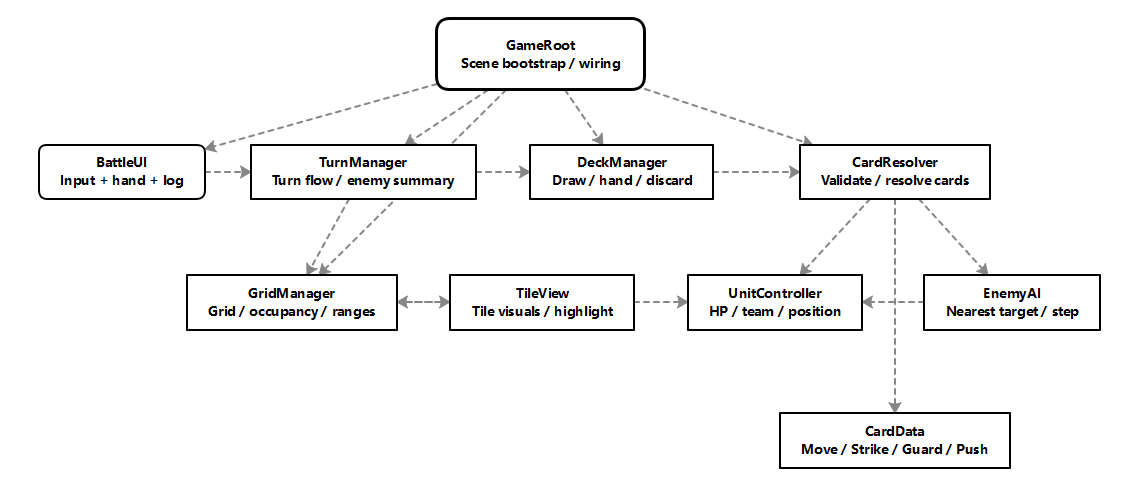
\includegraphics[width=\textwidth]{media/image2.png}
\caption{Tactical cards demo architecture}
\end{figure}

\subsection{Activity Diagram}

The gameplay loop diagram shows the main turn flow and battle progression of the demo.

\begin{figure}[H]
\centering
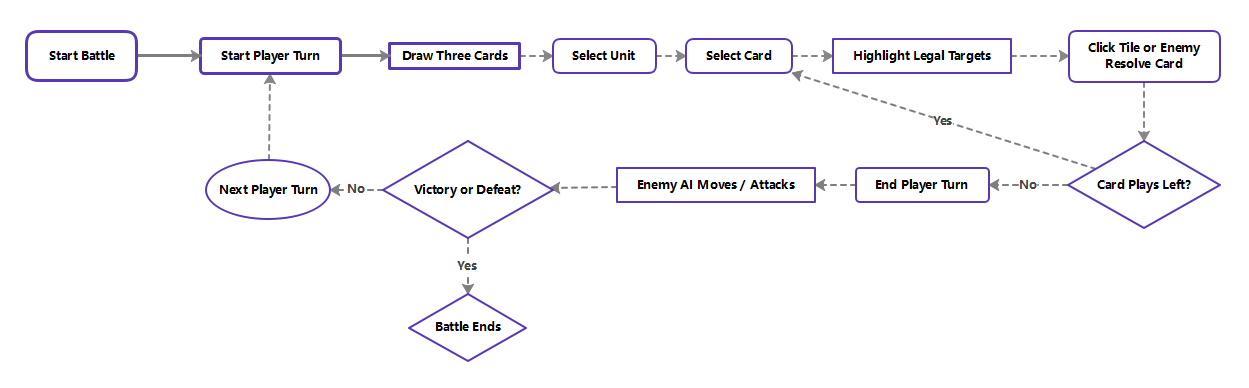
\includegraphics[width=\textwidth]{media/image4.png}
\caption{Gameplay loop}
\end{figure}

\subsection{Use Case Diagram}

At this stage, the core use cases are starting a battle, playing a card, moving a unit, attacking an enemy, defending a unit, ending the turn, viewing battle feedback, and observing the enemy turn. These use cases reflect the current gameplay goals rather than only the interface click sequence.

\begin{figure}[H]
\centering
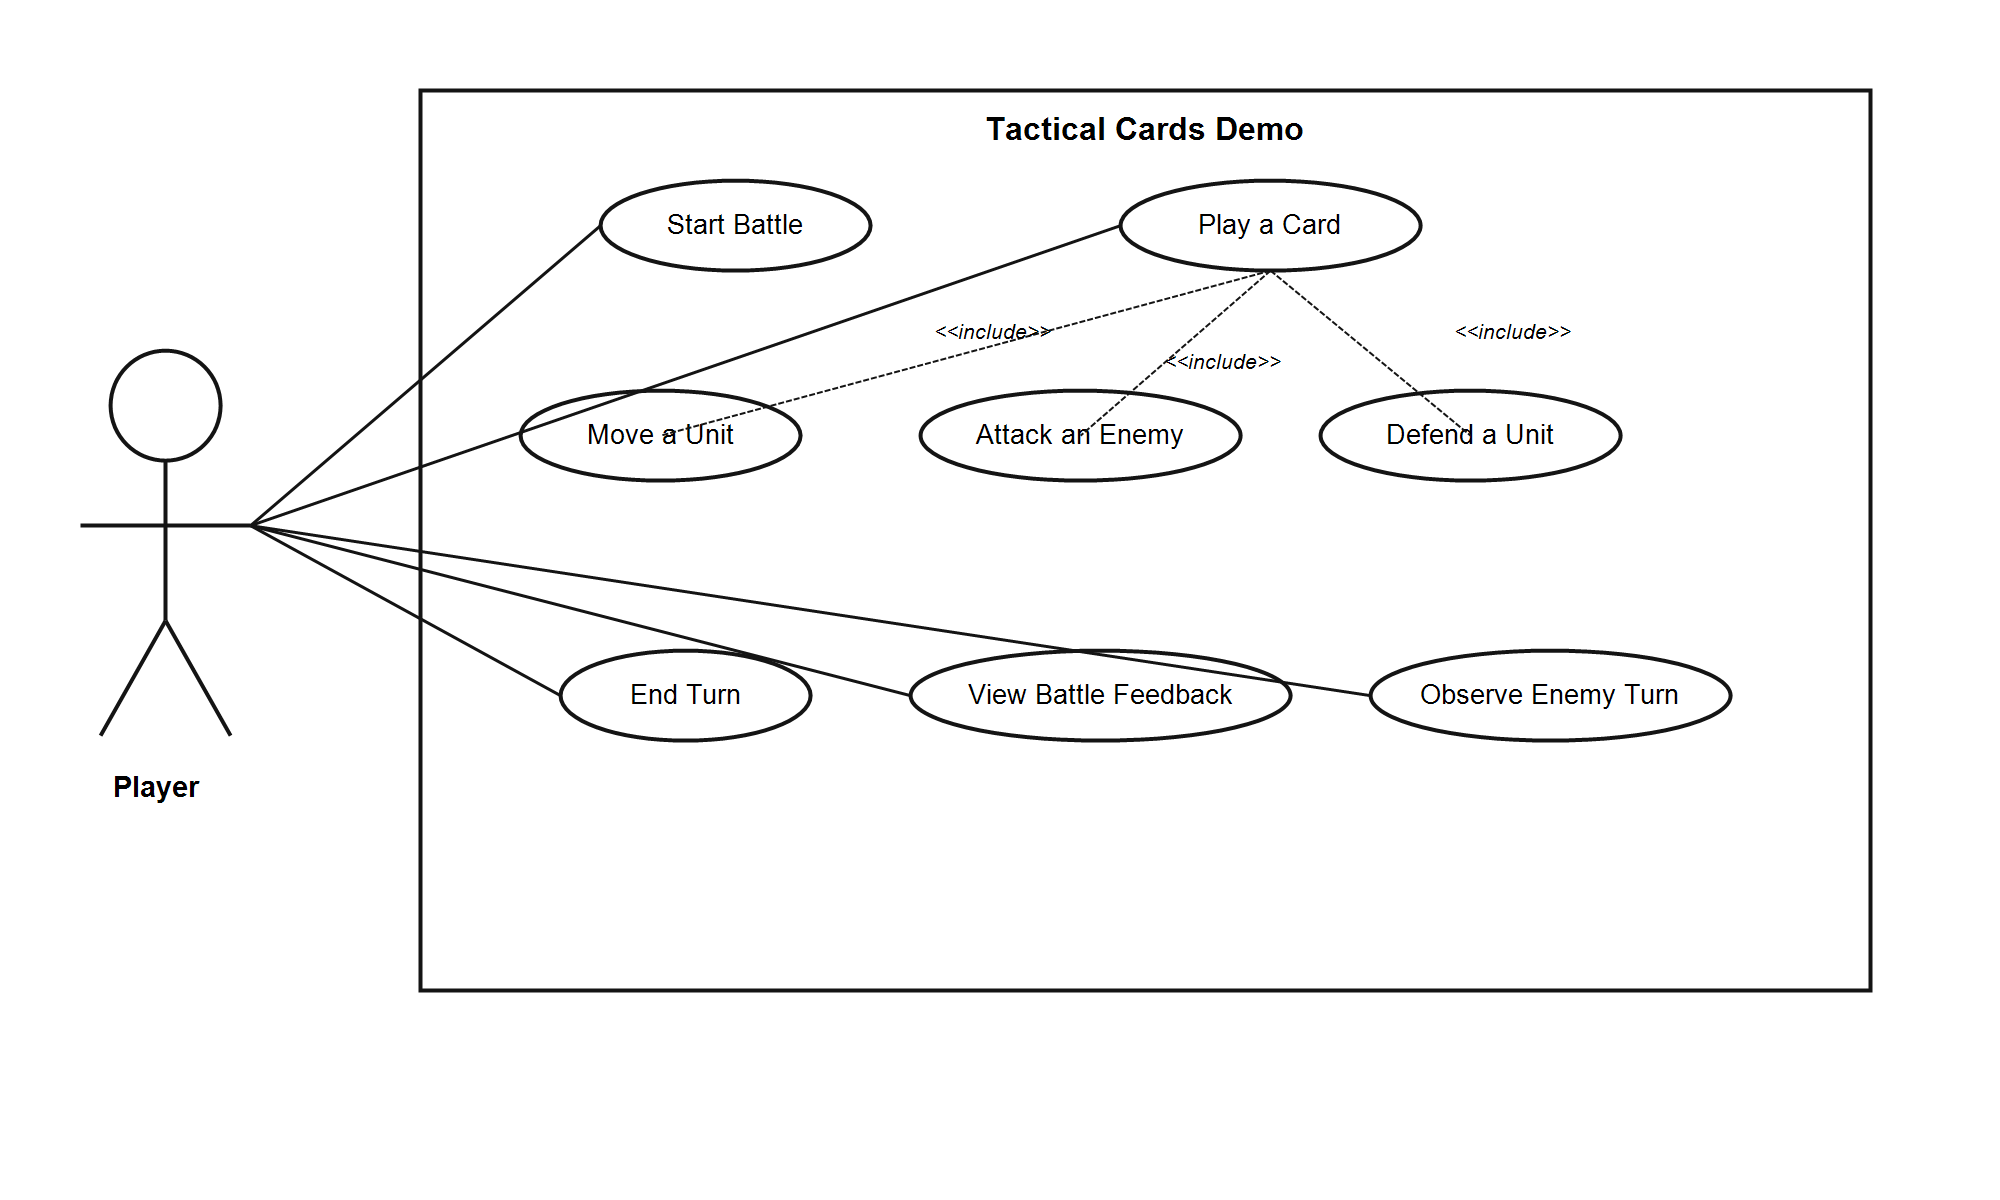
\includegraphics[width=\textwidth]{media/image6.png}
\caption{Use case diagram for the tactical cards demo}
\end{figure}

\subsection{State Diagram}

The unit state model shows the main combat-related states used in the demo design.

\begin{figure}[H]
\centering
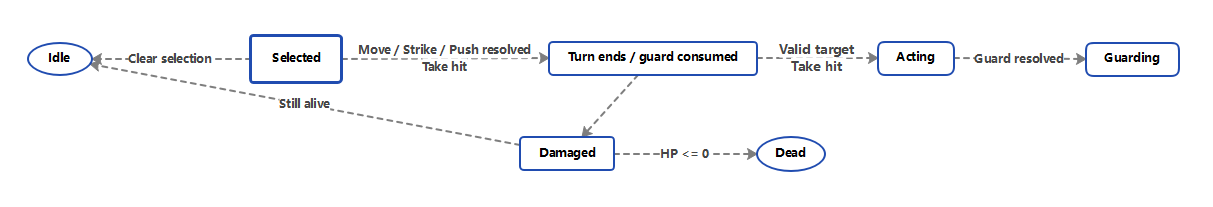
\includegraphics[width=\textwidth]{media/image3.png}
\caption{Unit state machine}
\end{figure}

\chapter{Summary and Reflections}

\section{Team Members and the Division of Labor}

\begin{itemize}
\item Guangjun HU: Requirements analysis, documentation
\item Hongshuo HU: Modeling, coding
\item Cheng YE: Coding, documentation
\item Zehan CHEN: Testing, web development
\end{itemize}

\section{Completed Process}

Set up a GitHub repository: \url{https://github.com/hu-zlatan/COMP4135-Group2-Project.git}

Specified the naming standards for file management as shown in Figure 4: \texttt{(Version Number)\_(Name of the file)\_(Editor)\_(Comment)}

\begin{figure}[H]
\centering
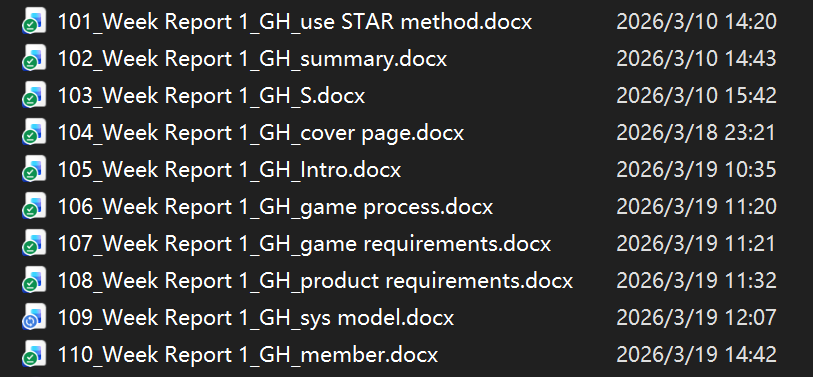
\includegraphics[width=0.7\textwidth]{media/image5.png}
\caption{File management sample}
\end{figure}

Assigned approximate role and tasks to each person.

Determined the basic game format.

\section{Future Plan}

Gradually carry out the development of the demo and form a game development requirements document. Manage the Git repository, conduct development on the develop branch, and merge tested versions into the main branch. Record bugs and form a bug library file. Maintain the meeting frequency to align ideas and requirements.

\chapter*{Reference}
\addcontentsline{toc}{chapter}{Reference}

\begin{enumerate}
\item COMP4135-CW1-Specification.
\item COMP4135 Week 3 Seminar Materials.
\item COMP4135 Week 4 Seminar Materials.
\end{enumerate}

\appendix
\chapter{Meeting Minutes}

\section{Meeting 1}

\textbf{Time}

3.17

\textbf{Attendance}

\begin{itemize}
\item Guangjun HU
\item Hongshuo HU
\item Zehan CHE
\end{itemize}

\textbf{Context}

Understand everyone's game ideas and interests, determine the division of labor, and define the game direction. Assign tasks and set the deadlines and delivery requirements for individual tasks.

\textbf{Decisions}

Project direction was confirmed as Tactical Cards, initial role allocation was agreed, and individual task expectations were set.

\textbf{Owner}

Guangjun HU, Hongshuo HU, and Zehan CHEN, with follow-up input from Cheng YE.

\textbf{Deadline}

18/03/2026 to 19/03/2026 for the initial WR1 materials and task allocation.

\textbf{Follow-up}

Reflected in the project direction, division of labour, and requirements sections of WR1.

\section{Meeting 2}

\textbf{Time}

3.18

\textbf{Attendance}

\begin{itemize}
\item Guangjun HU
\item Cheng YE
\end{itemize}

\textbf{Context}

Introduce the current situation, align the requirements, assign tasks and set the delivery time. To standardize the project communication and ensure all meeting information is traceable, the team has defined a unified meeting minutes format to be used for all subsequent project meetings. The format includes the following core sections:

\begin{enumerate}
\item \textbf{Basic Meeting Info}: Time, location (online/offline platform), attendance (present/absent/leave), recorder
\item \textbf{Agenda}: Pre-determined discussion topics and priority order
\item \textbf{Key Discussion Points}: Detailed notes of core content discussed for each agenda item, including different opinions, decision-making processes and final conclusions
\item \textbf{Action Items}: Assigned tasks, responsible person, expected delivery time, delivery standard and follow-up reviewer
\item \textbf{Open Issues}: Unresolved problems, pending discussion topics and required preparation work for the next meeting
\item \textbf{Next Meeting Arrangement}: Tentative time, main agenda and pre-work requirements for all members
\end{enumerate}

\textbf{Decisions}

The current requirements scope was aligned around a tactical card battle demo, UML diagram production was assigned, and a unified meeting-minutes format was defined for subsequent meetings.

\textbf{Owner}

Guangjun HU and Cheng YE, with follow-up support from the whole team.

\textbf{Deadline}

19/03/2026 for WR1 alignment; next weekly cycle for applying the meeting-minutes template.

\textbf{Follow-up}

Reflected in WR1 requirements, UML diagrams, and the team documentation process for later reports.

\end{document}
